%%%%%%%%%%%%%%%%%%%%%%%%%%%%%%%%%%%%%%%%%%%%%%%%%%%%%%%%%%%%%%%%%%%%%%%%%%%%%%%%
%2345678901234567890123456789012345678901234567890123456789012345678901234567890
%        1         2         3         4         5         6         7         8
% Comment this line out
                                                          % if you need a4paper
\documentclass[a4paper, 10pt, conference]{IEEEconf}    
\usepackage[utf8]{vietnam}
\usepackage{graphicx} 
\graphicspath{ {./images/} }
\title{\LARGE \bf
The Gooogle File System
}



\author{Huibert Kwakernaak$^{1}$ and Pradeep Misra$^{2}$% <-this % stops a space
\thanks{*This work was not supported by any organization}% <-this % stops a space
\thanks{$^{1}$H. Kwakernaak is with Faculty of Electrical Engineering, Mathematics and Computer Science,
        University of Twente, 7500 AE Enschede, The Netherlands
        {\tt\small h.kwakernaak at papercept.net}}%
\thanks{$^{2}$P. Misra is with the Department of Electrical Engineering, Wright State University,
        Dayton, OH 45435, USA
        {\tt\small p.misra at ieee.org}}%
}


\begin{document}



\maketitle
\thispagestyle{empty}
\pagestyle{empty}


%%%%%%%%%%%%%%%%%%%%%%%%%%%%%%%%%%%%%%%%%%%%%%%%%%%%%%%%%%%%%%%%%%%%%%%%%%%%%%%%
\begin{abstract}
Bài viết này giới thiệu về nền tảng lưu trữ của google, hệ thống Google File System. Google File System (GFS) là một hệ thống file lưu trữ phân tán - Distributed File System (DFS), được thiết kế và xây dựng để phục vụ một số lượng lớn các ứng dụng phân tán có cường độ trao đổi dữ liệu cao. GFS có tính chịu lỗi - fault tolerance ngay cả khi nó được triển khai trên môi trường phần cứng phổ thông, không chuyên dụnng, đồng thời, Hệ thống GFS cung cấp một hiệu năng tổng thể cao cho cho một lượng lớn các ứng dụng đóng vai trò client, sử dụng GFS để lưu trữ dữ liệu.

GFS được thiết kế với các mục đích giống với các hệ thống File System đã có trước đó, tuy nhiên, sự khác biệt của GFS so với các hệ thống cũ là ở chỗ, GFS được thiết kế dựa trên các đặc điểm hoạt động - trao đổi dữ liệu của các ứng dụng trong các hệ thống khác của Google có sử dụng GFS để lưu trữ dữ liệu. Bên cạnh đó, cơ sở thiết kế GFS cũng được dựa trên các đặc điểm của môi trường  công nghệ sẽ triển khai GFS của Google. Điều này có nghĩa rằng, GFS được thiết kế để phù hợp với môi trường hoạt động của Google, và được thiết kế nhằm phục vụ tốt nhất cho các ứng dụng của Google, chứ không phải nhằm hướng tới phục vụ cho mọi loại ứng dụng.

GFS được triển khai trên một quy mô lớn, phục vụ cho việc lưu trữ và xử lý dữ liệu của các Service trong hệ thống của Google. Bên cạnh đó, GFS cũng phục vụ cho các công việc nghiên cứu và phát triển các công nghệ có liên quan tới dữ liệu lớn. Cụm GFS cluster lớn nhất (tính tới thời điểm xuất bản bài báo) có kích thước hàng trăm terabyte, phân tán trên hàng ngàn ổ đĩa của hàng ngàn máy tính vật lý, và GFS cluster này có khả năng cùng một lúc cung cấp dịch vụ lưu trữ cho hàng trăm client, đáp ứng nhu cầu lưu trữ và xử lý dữ liệu của Google.

Bài viết này sẽ trình bày và thảo luận các khía cạnh khác nhau trong thiết kế của GFS, các tính năng mở rộng của GFS được thiết kế để phục vụ cho các ứng dụng phân tán. Sau đó, bài viết sẽ trình bày báo cáo về các đánh giá hiệu năng trên quy mô thử nghiệm - micro-benchmarks cũng như đánh giá hiệu năng trên môi trường sử dụng thực tế của Google.
\end{abstract}


%%%%%%%%%%%%%%%%%%%%%%%%%%%%%%%%%%%%%%%%%%%%%%%%%%%%%%%%%%%%%%%%%%%%%%%%%%%%%%%%
\section{Giới thiệu}
GFS được xây dựng để phục vụ nhu cầu lưu trữ và xử lý dữ liệu đang ngày càng gia tăng nhanh chóng của Google. Với mục đích này, GFS được thiết kế với các mục tiêu giống như các hệ thống Disttributed File System trước đó. Các mục tiêu mà GFS cần đạt được là hiệu năng, khả năng scaling, tính tin cậy, và tính sẵn sàng. Tuy nhiên, GFS được thiết kế để phục vụ cho Google, do đó GFS được thiết kế dựa trên cơ sở là các đặc điểm riêng của các ứng dụng Client trong hệ thống của Google, cũng như dựa trên các đặc điểm môi trường hệ thống phần cứng hiện có của Google. Chúng ta sẽ tìm hiểu chi tiết các đặc điểm riêng của các ứng dụng Client của Google là gì, để hiểu được tại sao những đặc điểm này lại tạo ra  những sự khác biệt giữa thiết kế của GFS với các hệ thống DFS trước đó.

Đầu tiên, thiết kế của GFS được dựa trên đặc điểm bất cứ thành phần nào ( kể cả phần cứng lẫn phần mềm) trong hệ thống GFS có thể xảy ra hỏng hóc, và sự hỏng hóc của các thành phần trong hệ thống được coi là một sự kiện thường xuyên xảy ra, và có thể xảy ra tại bất kỳ thời điểm nào, chứ không phải là một sự cố đặc biệt. GFS được thiết kế để triển khai trên môi trường phần cứng bao gồm hàng nghìn máy tính vật lý được dùng để lưu trữ dữ liệu. Các máy tính này có cấu hình phần cứng phổ thông, do đó chúng ta khồng đảm bảo về chất lượng của phần cứng các máy tính này. Điều này dẫn tới việc một số phần cứng, phần mềm trên các máy tính này có thể xảy ra sự cố và hỏng hóc. Và khi sự cố xảy ra, những dữ liệu lưu trữ trên các máy tính bị hỏng sẽ có khả năng bị mất và không thể phục hồi được. Các lỗi phần cứng, phần mềm trên các máy tính của hệ thống có thể xảy ra do nhiều nguồn khác nhau gây ra như: Bug của phần mềm, hệ điều hành gặp sự cố, lỗi do con người gây ra, lỗi ổ đĩa cứng, lỗi RAM, lỗi mạng và lỗi do hệ thống điện. Để giải quyết vấn đề các thành phần trên hệ thống gặp sự cố, hệ thống GFS phải xây dựng và tích hợp các cơ chế kiểm soát, theo dõi toàn bộ các thành phần trong hệ thống, cơ chế phát hiện lỗi, cơ chế chống lỗi, cũng như cơ chế phục hồi các thành phần bị lỗi khi sự cố xảy ra.

Thứ hai, đa số các file được lưu trữ và xử lý trong hệ thống GFS có đặc điểm là có kích thước rất lớn, lên tới kích cỡ hàng GB. Mỗi một file có nội dung bao gồm rất nhiều các object của các ứng dụng, ví dụ như một file dữ liệu có thể chứa tới hàng nghìn các trang web. Lý do để gom hàng nghìn object vào một file như vậy, là vì khi làm việc với hàng tỉ object có kích thước hàng nghìn TB như vậy, việc lưu trữ mỗi một object vào một file làm giảm hiệu năng của hệ thống, vì quá trình quản lý cũng như băng thông I/O của hệ thống có hàng tỉ file có kích thước nhỏ là chậm và không hiệu quả bằng một hệ thống có các file có kích thước lớn và số lượng file nhỏ.

Thứ ba, nội dung của đa số các file trong hệ thống GFS được thay đổi bằng cách chèn thêm dữ liệu mới (append) thay vì ghi đè (overwriting) dữ liệu cũ. Việc thay đổi file bằng cách ghi ngẫu nhiên là hầu như không xảy ra. Đồng thời, hoạt động chủ yếu của hệ thống khi tương tác với các file là hoạt động đọc dữ liệu của file, và hầu hết các Client khi đọc các file lưu trữ trong GFS đều đọc theo kiểu đọc tuần tự - sequentially read. GFS có đặc điểm trên, là do nhiều ứng dụng xử lý dữ liệu của Google đọc dữ liệu bằng cách quét tuần tự qua một file. Đồng thời, rất nhiều file trong hệ thống của Google được tạo ra bằng cách streamming dữ liệu, ví dụ như truyền video, hay crawl web,... Một số lượng lớn dữ liệu tồn tại dưới dạng file nén, một số file là kết quả của việc nhiều máy tính cùng ghi dữ liệu vào file đó một lúc, hoặc được ghi vào trong nhiều thời điểm khác nhau. Với các đặc điểm về phương thức tương tác, sử dụng các file trong hệ thống GFS của các ứng dụng Client trong hệ thống Google như vậy, cùng với việc các file trong GFS thường có kích thước rất lớn, thì việc thiết kế hệ thống sẽ tập trung vào thao tác nạp thêm dữ liệu vào file (data append) cho phép hệ thống đạt được hiện năng tối ưu, cũng như đảm bảo tính toàn vẹn (atomicity) của record dữ liệu được append vào. Đồng thời, việc sử dụng thao tác append để thêm dữ liệu vào một file cho phép chúng ta không cần thiết kế các bộ đệm dữ liệu ở phía Client nữa.
\begin{figure*}
  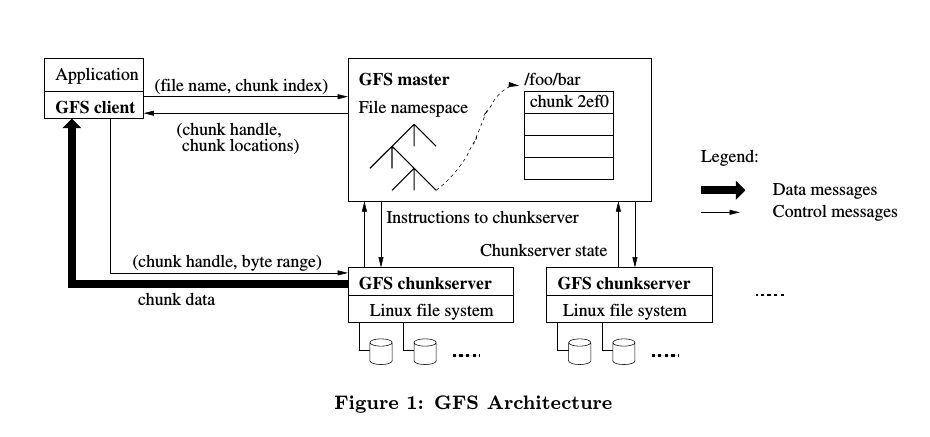
\includegraphics[width=\textwidth,height=8cm]{GFS-Architecture.png}
  \caption{GFS Architect}
\end{figure*}
Thứ tư, song song với việc GFS được thiết kế để phục vụ tốt nhất cho các ứng dụng của Google, thì Google cũng thiết kế các thư viện, API riêng cho các ứng dụng Client, để hỗ trợ các ứng dụng Client này có thể tương tác, trao đổi dữ liệu với GFS một cách hiệu quả, đồng thời tăng tính mềm dẻo của toàn bộ hệ thống (bao gồm cả GFS lẫn các Client application). Bên cạnh đó, việc GFS sử dụng mô hình nhất quán có tính mềm dẻo là relaxed consistency model (sẽ được trình bày ở phần 2.7) cho phép chúng ta đơn giản hóa thiết kế của hệ thống GFS mà không làm phần xử lý bên phía Client phức tạp lên, nhưng vẫn đảm bảo dữ liệu của chúng ta có mức độ nhất quán phù hợp với yêu cầu của ứng dụng Client. Bên cạnh đó, so với các hệ thống file trước kia, GFS có thêm một thao tác thay đổi dữ liệu mới, đó là thao tác record append. Với thao tác này, GFS cho phép nhiều ứng dụng có thể chèn thêm các record dữ liệu vào cùng một file đồng thời với nhau mà không cần phải thực hiện thêm việc đồng bộ hóa giữa các ứng dụng này. Thao tác data append trong GFS sẽ còn được thảo luận thêm trong phần sau của bài viết.

Hàng loạt GFS cluster đã được triển khai để phục vụ các mục đích khác nhau của Google. GFS cluster lớn nhất có hơn 1000 node, chứa 300 TB dữ liệu và phục vụ cho hàng trăm ứng dụng client cùng một lúc.


\section{Tổng quan về thiết kế của GFS}

\subsection{Các giả thiết được sử dụng làm cơ sở để xây dựng GFS}

Để thực hiện việc thiết kế hệ thống GFS, các nhà phát triển của Google đã đặt ra một số giả thiết làm điều kiện tiền đề cho hệ thống. Các giả thiết này được đặt ra dựa trên những đặc điểm về ứng dụng sử dụng cũng như các đặc điểm về hệ thống phần cứng triển khai GFS mà chúng ta đã nêu ra ở phần giới thiệu. Sự có mặt của các giả thiết này vừa đặt ra những thách thức, vừa đem tới các yếu tố thuận lợi cho việc thiết kế GFS. Các giả thiết ở đây là:

- GFS được triển khai trên môi trường hệ thống được xây dựng từ các thành phần phần cứng phổ thông, vì vậy các thành phần trong hệ thống có thể thường xuyên xảy ra lỗi. GFS phải có khả năng thao dõi và phát hiện ra các thành phần nào trong hệ thống đang gặp lỗi, đồng thời GFS vẫn phải có khả năng hoạt động bình thường ngay cả khi một số hoạt động đang gặp lỗi, và sau khi phát hiển ra các thành phần lỗi GFS phải nhanh chóng phục hồi các dữ liệu đã bị mất trên các thành phần này.

- Phần lớn các file được lưu trữ và xử lý bởi GFS là các file có kích thước lớn. Số lượng file được lưu trữ trong hệ thống là khoảng vài triệu file, với kích thước của một file thường lớn hơn 100 MB. Do số lượng các file có kích cỡ hàng GB trong hệ thống GFS là lớn, do đó chúng ta có thể thấy GFS sẽ cần tập trung để tối ưu hóa cho việc quản lý, truy cập và xử lý các file có kích thước lớn. Bên cạnh đó, GFS vẫn cho phép các client application làm việc với các file có kích thước nhỏ, tuy nhiên hệ thống GFS sẽ không tối ưu cho các file có kích thước nhỏ này.

- Khối lượng công việc (workload) mà các Client application đặt lên hệ thống lưu trữ GFS do chủ yếu 2 thao tác sau gây ra: Streaming read - đọc theo luồng và random read - đọc ngẫu nhiên. Thao tác streaming read được sử dụng để đọc một lượng nhỏ dữ liệu một lần (vài trăm KB - 1MB), nhưng số lần đọc là rất lớn, và dữ liệu ở các lần đọc liên tiếp nhau cũng nằm liên tiếp nhau ( do vậy thao tác đọc này được gọi là streaming). Thao tác random read thường đọc một lượng nhỏ dữ liệu ở một vị trí nào đó trong file. Các ứng dụng cần có hiệu năng trao đổi dữ liệu cao thường gom nhóm các yêu cầu đọc của nó vào và sắp xếp các yêu cầu đọc đó theo thứ tự rồi mới gửi lần lượt các yêu cầu đọc tới GFS, việc này giúp thao tác đọc dữ liệu của ứng dụng đó diễn ra theo cách tuần tự - sequential read, qua đó giúp hiệu năng của thao tác đọc dữ liệu qua GFS tăng lên.

- Bên cạnh 2 thao tác đọc trên, các ứng dụng client cũng trao đổi một khối lượng lớn dữ liệu với GFS thông qua một lượng lớn các thao tác write-append. Điểm đặc biệt của thao tác write-append là thao tác này nạp dữ liệu vào cuối của file, chứ không phải là ghi đè dữ liệu vào một offset trước đó của file. Kích thước dữ liệu mà mỗi thao tác write-append ghi thêm vào cuối file tương tự như kích thước dữ liệu mà thao tác streaming read đọc được mỗi lần (vài trăm KB - 1 MB). Thao tác ghi dữ liệu vào một vị trí trong file (write) vẫn được được GFS hỗ trợ, tuy nhiên GFS sẽ không tối ưu hiệu năng cho thao tác này.

- Hệ thống GFS cần xây dựng cơ chế cho phép một số lượng lớn các client có thể đồng thời (concurrently) thực hiện thao tác write-append vào cùng một file với nhau. Yêu cầu này được đặt ra,vì trong qúa trình sử dụng thực tế, trong hệ thống Google, sẽ thường xuyên xảy ra trường hợp có hàng trăm client cùng 1 lúc thực hiện thao tác write-append vào một file trong GFS. Bên cạnh việc cho phép các thao tác trên được thực hiện đồng thời, chúng ta vẫn cần đảm bảo các thao tác write-append này được đồng bộ hóa với nhau,vơi điều kiện là khi thực hiện việc đồng bộ các thao tác append, sự quá tải gây ra trên hệ thống là nhỏ nhất.

- Trong hệ thống sử dụng GFS, hệ thống mạng sẽ ưu tiên tối ưu sao cho băng thông của mạng cao, hơn là tạo ra độ trễ thấp, vì đa số các ứng dụng sử dụng GFS cần tốc độ xử lý - truyền tải dữ liệu cao (cần có băng thông cao) hơn là thời gian phản hồi của GFS cho một yêu cầu đọc/ghi thấp (cần có độ trễ thấp).

\subsection{Maintaining the Integrity of the Specifications}

The template is used to format your paper and style the text. All margins, column widths, line spaces, and text fonts are prescribed; please do not alter them. You may note peculiarities. For example, the head margin in this template measures proportionately more than is customary. This measurement and others are deliberate, using specifications that anticipate your paper as one part of the entire proceedings, and not as an independent document. Please do not revise any of the current designations

\section{MATH}

Before you begin to format your paper, first write and save the content as a separate text file. Keep your text and graphic files separate until after the text has been formatted and styled. Do not use hard tabs, and limit use of hard returns to only one return at the end of a paragraph. Do not add any kind of pagination anywhere in the paper. Do not number text heads-the template will do that for you.

Finally, complete content and organizational editing before formatting. Please take note of the following items when proofreading spelling and grammar:

\subsection{Abbreviations and Acronyms} Define abbreviations and acronyms the first time they are used in the text, even after they have been defined in the abstract. Abbreviations such as IEEE, SI, MKS, CGS, sc, dc, and rms do not have to be defined. Do not use abbreviations in the title or heads unless they are unavoidable.

\subsection{Units}

\begin{itemize}

\item Use either SI (MKS) or CGS as primary units. (SI units are encouraged.) English units may be used as secondary units (in parentheses). An exception would be the use of English units as identifiers in trade, such as Ò3.5-inch disk driveÓ.
\item Avoid combining SI and CGS units, such as current in amperes and magnetic field in oersteds. This often leads to confusion because equations do not balance dimensionally. If you must use mixed units, clearly state the units for each quantity that you use in an equation.
\item Do not mix complete spellings and abbreviations of units: ÒWb/m2Ó or Òwebers per square meterÓ, not Òwebers/m2Ó.  Spell out units when they appear in text: Ò. . . a few henriesÓ, not Ò. . . a few HÓ.
\item Use a zero before decimal points: Ò0.25Ó, not Ò.25Ó. Use Òcm3Ó, not ÒccÓ. (bullet list)

\end{itemize}


\subsection{Equations}

The equations are an exception to the prescribed specifications of this template. You will need to determine whether or not your equation should be typed using either the Times New Roman or the Symbol font (please no other font). To create multileveled equations, it may be necessary to treat the equation as a graphic and insert it into the text after your paper is styled. Number equations consecutively. Equation numbers, within parentheses, are to position flush right, as in (1), using a right tab stop. To make your equations more compact, you may use the solidus ( / ), the exp function, or appropriate exponents. Italicize Roman symbols for quantities and variables, but not Greek symbols. Use a long dash rather than a hyphen for a minus sign. Punctuate equations with commas or periods when they are part of a sentence, as in

$$
\alpha + \beta = \chi \eqno{(1)}
$$

Note that the equation is centered using a center tab stop. Be sure that the symbols in your equation have been defined before or immediately following the equation. Use Ò(1)Ó, not ÒEq. (1)Ó or Òequation (1)Ó, except at the beginning of a sentence: ÒEquation (1) is . . .Ó

\subsection{Some Common Mistakes}
\begin{itemize}


\item The word ÒdataÓ is plural, not singular.
\item The subscript for the permeability of vacuum ?0, and other common scientific constants, is zero with subscript formatting, not a lowercase letter ÒoÓ.
\item In American English, commas, semi-/colons, periods, question and exclamation marks are located within quotation marks only when a complete thought or name is cited, such as a title or full quotation. When quotation marks are used, instead of a bold or italic typeface, to highlight a word or phrase, punctuation should appear outside of the quotation marks. A parenthetical phrase or statement at the end of a sentence is punctuated outside of the closing parenthesis (like this). (A parenthetical sentence is punctuated within the parentheses.)
\item A graph within a graph is an ÒinsetÓ, not an ÒinsertÓ. The word alternatively is preferred to the word ÒalternatelyÓ (unless you really mean something that alternates).
\item Do not use the word ÒessentiallyÓ to mean ÒapproximatelyÓ or ÒeffectivelyÓ.
\item In your paper title, if the words Òthat usesÓ can accurately replace the word ÒusingÓ, capitalize the ÒuÓ; if not, keep using lower-cased.
\item Be aware of the different meanings of the homophones ÒaffectÓ and ÒeffectÓ, ÒcomplementÓ and ÒcomplimentÓ, ÒdiscreetÓ and ÒdiscreteÓ, ÒprincipalÓ and ÒprincipleÓ.
\item Do not confuse ÒimplyÓ and ÒinferÓ.
\item The prefix ÒnonÓ is not a word; it should be joined to the word it modifies, usually without a hyphen.
\item There is no period after the ÒetÓ in the Latin abbreviation Òet al.Ó.
\item The abbreviation Òi.e.Ó means Òthat isÓ, and the abbreviation Òe.g.Ó means Òfor exampleÓ.

\end{itemize}


\section{USING THE TEMPLATE}

Use this sample document as your LaTeX source file to create your document. Save this file as {\bf root.tex}. You have to make sure to use the cls file that came with this distribution. If you use a different style file, you cannot expect to get required margins. Note also that when you are creating your out PDF file, the source file is only part of the equation. {\it Your \TeX\ $\rightarrow$ PDF filter determines the output file size. Even if you make all the specifications to output a letter file in the source - if you filter is set to produce A4, you will only get A4 output. }

It is impossible to account for all possible situation, one would encounter using \TeX. If you are using multiple \TeX\ files you must make sure that the ``MAIN`` source file is called root.tex - this is particularly important if your conference is using PaperPlaza's built in \TeX\ to PDF conversion tool.

\subsection{Headings, etc}

Text heads organize the topics on a relational, hierarchical basis. For example, the paper title is the primary text head because all subsequent material relates and elaborates on this one topic. If there are two or more sub-topics, the next level head (uppercase Roman numerals) should be used and, conversely, if there are not at least two sub-topics, then no subheads should be introduced. Styles named ÒHeading 1Ó, ÒHeading 2Ó, ÒHeading 3Ó, and ÒHeading 4Ó are prescribed.

\subsection{Figures and Tables}

Positioning Figures and Tables: Place figures and tables at the top and bottom of columns. Avoid placing them in the middle of columns. Large figures and tables may span across both columns. Figure captions should be below the figures; table heads should appear above the tables. Insert figures and tables after they are cited in the text. Use the abbreviation ÒFig. 1Ó, even at the beginning of a sentence.

\begin{table}[h]
\caption{An Example of a Table}
\label{table_example}
\begin{center}
\begin{tabular}{|c||c|}
\hline
One & Two\\
\hline
Three & Four\\
\hline
\end{tabular}
\end{center}
\end{table}


   \begin{figure}[thpb]
      \centering
      \framebox{\parbox{3in}{We suggest that you use a text box to insert a graphic (which is ideally a 300 dpi TIFF or EPS file, with all fonts embedded) because, in an document, this method is somewhat more stable than directly inserting a picture.
}}
      %\includegraphics[scale=1.0]{figurefile}
      \caption{Inductance of oscillation winding on amorphous
       magnetic core versus DC bias magnetic field}
      \label{figurelabel}
   \end{figure}
   

Figure Labels: Use 8 point Times New Roman for Figure labels. Use words rather than symbols or abbreviations when writing Figure axis labels to avoid confusing the reader. As an example, write the quantity ÒMagnetizationÓ, or ÒMagnetization, MÓ, not just ÒMÓ. If including units in the label, present them within parentheses. Do not label axes only with units. In the example, write ÒMagnetization (A/m)Ó or ÒMagnetization {A[m(1)]}Ó, not just ÒA/mÓ. Do not label axes with a ratio of quantities and units. For example, write ÒTemperature (K)Ó, not ÒTemperature/K.Ó

\section{CONCLUSIONS}

A conclusion section is not required. Although a conclusion may review the main points of the paper, do not replicate the abstract as the conclusion. A conclusion might elaborate on the importance of the work or suggest applications and extensions. 

\addtolength{\textheight}{-12cm}   % This command serves to balance the column lengths
                                  % on the last page of the document manually. It shortens
                                  % the textheight of the last page by a suitable amount.
                                  % This command does not take effect until the next page
                                  % so it should come on the page before the last. Make
                                  % sure that you do not shorten the textheight too much.

%%%%%%%%%%%%%%%%%%%%%%%%%%%%%%%%%%%%%%%%%%%%%%%%%%%%%%%%%%%%%%%%%%%%%%%%%%%%%%%%



%%%%%%%%%%%%%%%%%%%%%%%%%%%%%%%%%%%%%%%%%%%%%%%%%%%%%%%%%%%%%%%%%%%%%%%%%%%%%%%%



%%%%%%%%%%%%%%%%%%%%%%%%%%%%%%%%%%%%%%%%%%%%%%%%%%%%%%%%%%%%%%%%%%%%%%%%%%%%%%%%
\section*{APPENDIX}

Appendixes should appear before the acknowledgment.

\section*{ACKNOWLEDGMENT}

The preferred spelling of the word ÒacknowledgmentÓ in America is without an ÒeÓ after the ÒgÓ. Avoid the stilted expression, ÒOne of us (R. B. G.) thanks . . .Ó  Instead, try ÒR. B. G. thanksÓ. Put sponsor acknowledgments in the unnumbered footnote on the first page.



%%%%%%%%%%%%%%%%%%%%%%%%%%%%%%%%%%%%%%%%%%%%%%%%%%%%%%%%%%%%%%%%%%%%%%%%%%%%%%%%

References are important to the reader; therefore, each citation must be complete and correct. If at all possible, references should be commonly available publications.



\begin{thebibliography}{99}

\bibitem{c1}  York: McGraw-Hill, 







\end{thebibliography}




\end{document}
